% From assignment:
% Prioritize measurements and analysis/interpretation!

% Demonstrate use of tools (profiling, ...) , and simple performance
% model.

\subsection{Compilation flags}

\begin{figure}[!htbp] \centering
  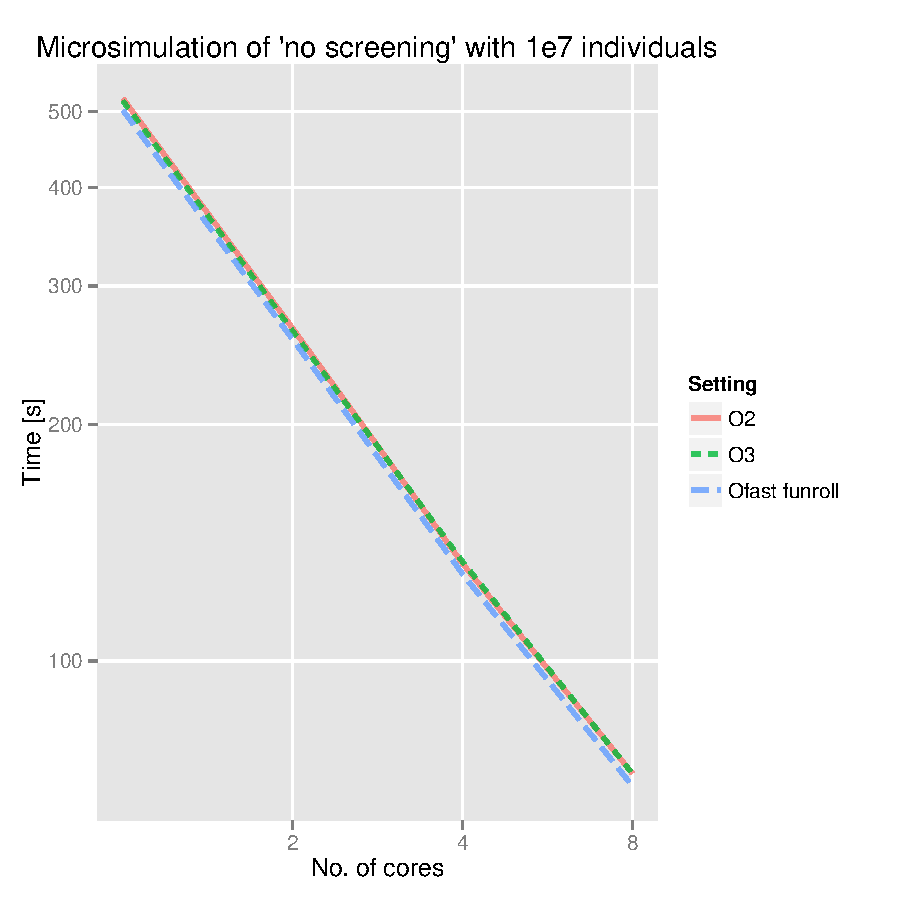
\includegraphics[height=0.5\textheight]{images/flagsProfiling.pdf}
  \caption{Performance effect of using the compilation flags
    \texttt{-O2}, \texttt{-O3} and \texttt{-Ofast -funroll-all-loops}
    for a number of cores. The black dashed line represents ideal
    scaling.}
  \label{fig:flagScaling}
\end{figure}

For the ``improved OpenMP'', we continued with investigating the
performance effect of compilation flags. For an R package the
\texttt{CXX} flags can be set in multiple ways. We first tried to change the R package
specific setting, in \texttt{/src/Makevars}, but for our settings to
take precedence over the Ferlin system settings we had to set the
flags in \texttt{$\sim$/.R/Makevars}. In Figure \ref{fig:flagScaling} we
compare the performance effect of using the compilation flags
\texttt{-O2}, \texttt{-O3} and \texttt{-Ofast -funroll-all-loops} for
a number of cores. The effect of setting compilation flags is small in
comparison to the effect of using multiple cores.

%%% Local Variables: 
%%% mode: latex 
%%% TeX-master: "report" 
%%% End:
